\documentclass[aspectratio=169,xcolor=table]{beamer}

% --- Pacchetti ---
\usepackage[utf8]{inputenc}
\usepackage[T1]{fontenc}
\usepackage[italian]{babel}
\usepackage{lmodern}
\usepackage{graphicx}
\usepackage{booktabs}
\usepackage{xcolor}
\usepackage{amsmath, amssymb}
\usepackage{tikz}
\usetikzlibrary{arrows.meta, positioning}

% --- Configurazione Tema (Madrid elegante con colore personalizzato) ---
\usetheme{Madrid}
\definecolor{unimeblue}{RGB}{12, 35, 64} % Blu scuro istituzionale
\usecolortheme[named=unimeblue]{structure}

% --- Informazioni ---
\title[Lab IA - Progetto 1]{Progetto 1: Segmentazione Clienti e Churn Prediction}
\subtitle{Spiegazione Semplificata del Progetto}
\author[Massimo Mantineo]{Massimo Mantineo\\{\small Matricola: 541924}}
\institute[Unime MIFT]{
  Università degli Studi di Messina\\
  Corso di Laurea in Informatica
}
\date[A.A. 2025/2026]{Laboratorio di Intelligenza Artificiale\\A.A. 2025/2026}

% Logo nel titolo
\titlegraphic{
\includegraphics[width=3cm]{logo_unime_orizontale.png}}

\begin{document}

% Slide 1: Titolo
\begin{frame}
  \titlepage
\end{frame}

% Slide 2: Obiettivi e Dataset
\begin{frame}{1. Di cosa tratta il Progetto e da dove vengono i Dati?}
  \begin{columns}
    \begin{column}{0.55\textwidth}
      \textbf{Il Dataset:}
      \begin{itemize}
        \item Usiamo il dataset reale \textbf{Telco Customer Churn di IBM}.
        \item Contiene i profili commerciali e anagrafici di 7043 clienti.
      \end{itemize}
      \vspace{0.2cm}
      \textbf{L'obiettivo:}
      \begin{itemize}
        \item Capire quali clienti rischiano di abbandonare l'operatore (\textbf{Churn Prediction}) per intervenire in tempo.
      \end{itemize}
      \vspace{0.2cm}
      \textbf{La sproporzione delle classi:}
      \begin{itemize}
        \item Le classi sono sbilanciate (3:1): 73.4\% fedeli e 26.6\% che abbandonano.
      \end{itemize}
    \end{column}
    \begin{column}{0.43\textwidth}
      \centering
      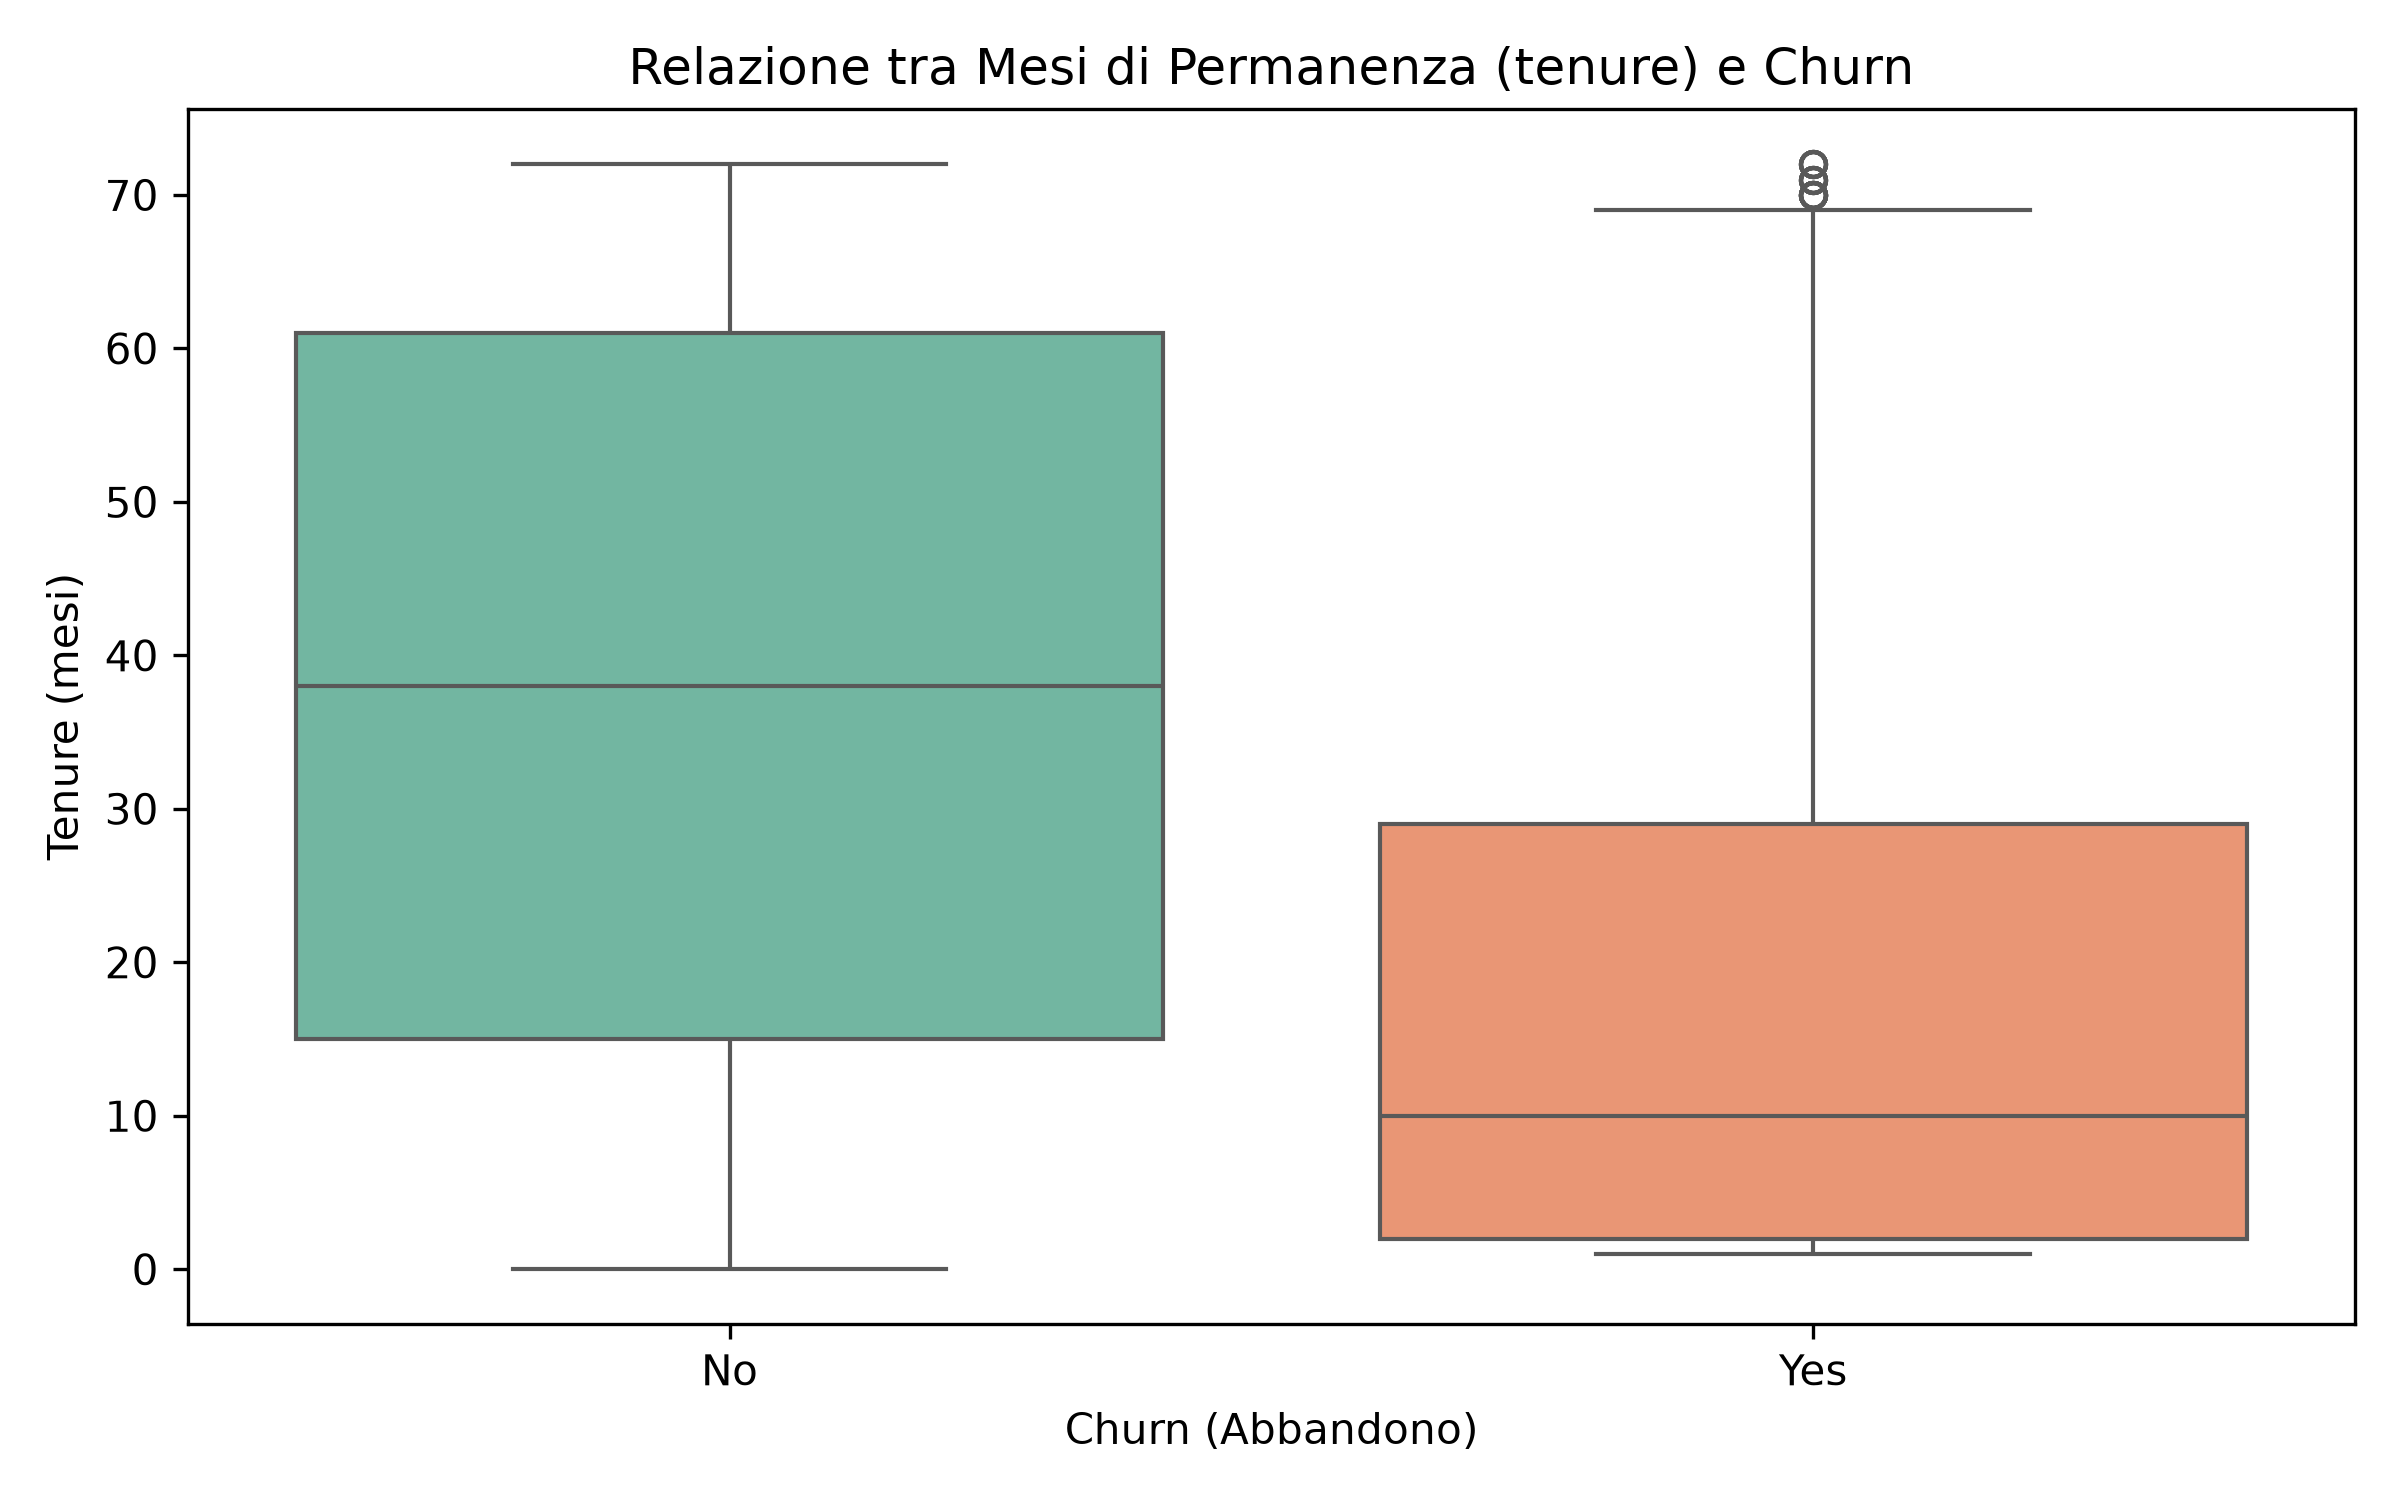
\includegraphics[width=0.9\textwidth]{../grafici/churn_vs_tenure.png}
      \begin{center}\scriptsize \textbf{Grafico}: Chi se ne va (Yes Churn) ha una permanenza bassissima (mediana $\approx$ 10 mesi).\end{center}
    \end{column}
  \end{columns}
\end{frame}

% Slide 3: Preprocessing dei Dati
\begin{frame}{2. Come abbiamo sistemato i Dati? (Preprocessing)}
  \centering
  \begin{tikzpicture}[
    node distance=0.8cm and 0.6cm,
    box/.style={
      rectangle,
      draw=unimeblue!80,
      fill=unimeblue!5,
      thick,
      rounded corners=4pt,
      text width=4.3cm,
      minimum height=1.8cm,
      align=center,
      font=\scriptsize
    },
    arrow/.style={
      -{Stealth[scale=1.2]},
      line width=1.5pt,
      orange!90!black
    }
  ]

    % Row 1
    \node[box] (b1) {
      \textbf{1. Celle Vuote}\\[0.1cm]
      Riempite 11 celle in \textit{TotalCharges} con \texttt{0.0} (nuovi clienti con \textit{tenure}=0) e convertito in float.
    };
    
    \node[box, right=of b1] (b2) {
      \textbf{2. Rimuovi ID}\\[0.1cm]
      Rimosso \textit{customerID} poiché privo di valore predittivo; evita l'overfitting.
    };
    
    \node[box, right=of b2] (b3) {
      \textbf{3. One-Hot Encoding}\\[0.1cm]
      Tradotte parole in 0/1. Usato \texttt{drop\_first=True} per evitare ridondanze.
    };

    % Row 2
    \node[box, below=0.8cm of b3] (b4) {
      \textbf{4. Splitting}\\[0.1cm]
      Diviso in Train (80\%) e Test (20\%) \textbf{prima} dello scaling per evitare \textit{Data Leakage}.
    };
    
    \node[box, left=of b4] (b5) {
      \textbf{5. Scaling}\\[0.1cm]
      Standard Scaling (media 0, dev. std. 1) per uniformare la scala delle variabili.
    };

    % Connections
    \draw[arrow] (b1) -- (b2);
    \draw[arrow] (b2) -- (b3);
    \draw[arrow] (b3) -- (b4);
    \draw[arrow] (b4) -- (b5);

  \end{tikzpicture}
\end{frame}

% Slide 4: Apprendimento Non Supervisionato (Clustering k-Means)
\begin{frame}{3. Segmentazione dei Clienti (Clustering k-Means)}
  \begin{columns}
    \begin{column}{0.48\textwidth}
      \textbf{Scelta del numero di Cluster ($k$):}
      \vspace{0.1cm}
      \begin{itemize}
        \item \textbf{Inertia (Gomito)}: Indica compattezza dei gruppi. La curva flette a $k=2$ e $k=3$.
        \item \textbf{Silhouette Score}: Indica separazione. Raggiunge il suo \textbf{massimo assoluto a $k=2$ (0.2946)}.
      \end{itemize}
      \vspace{0.1cm}
      \centering
      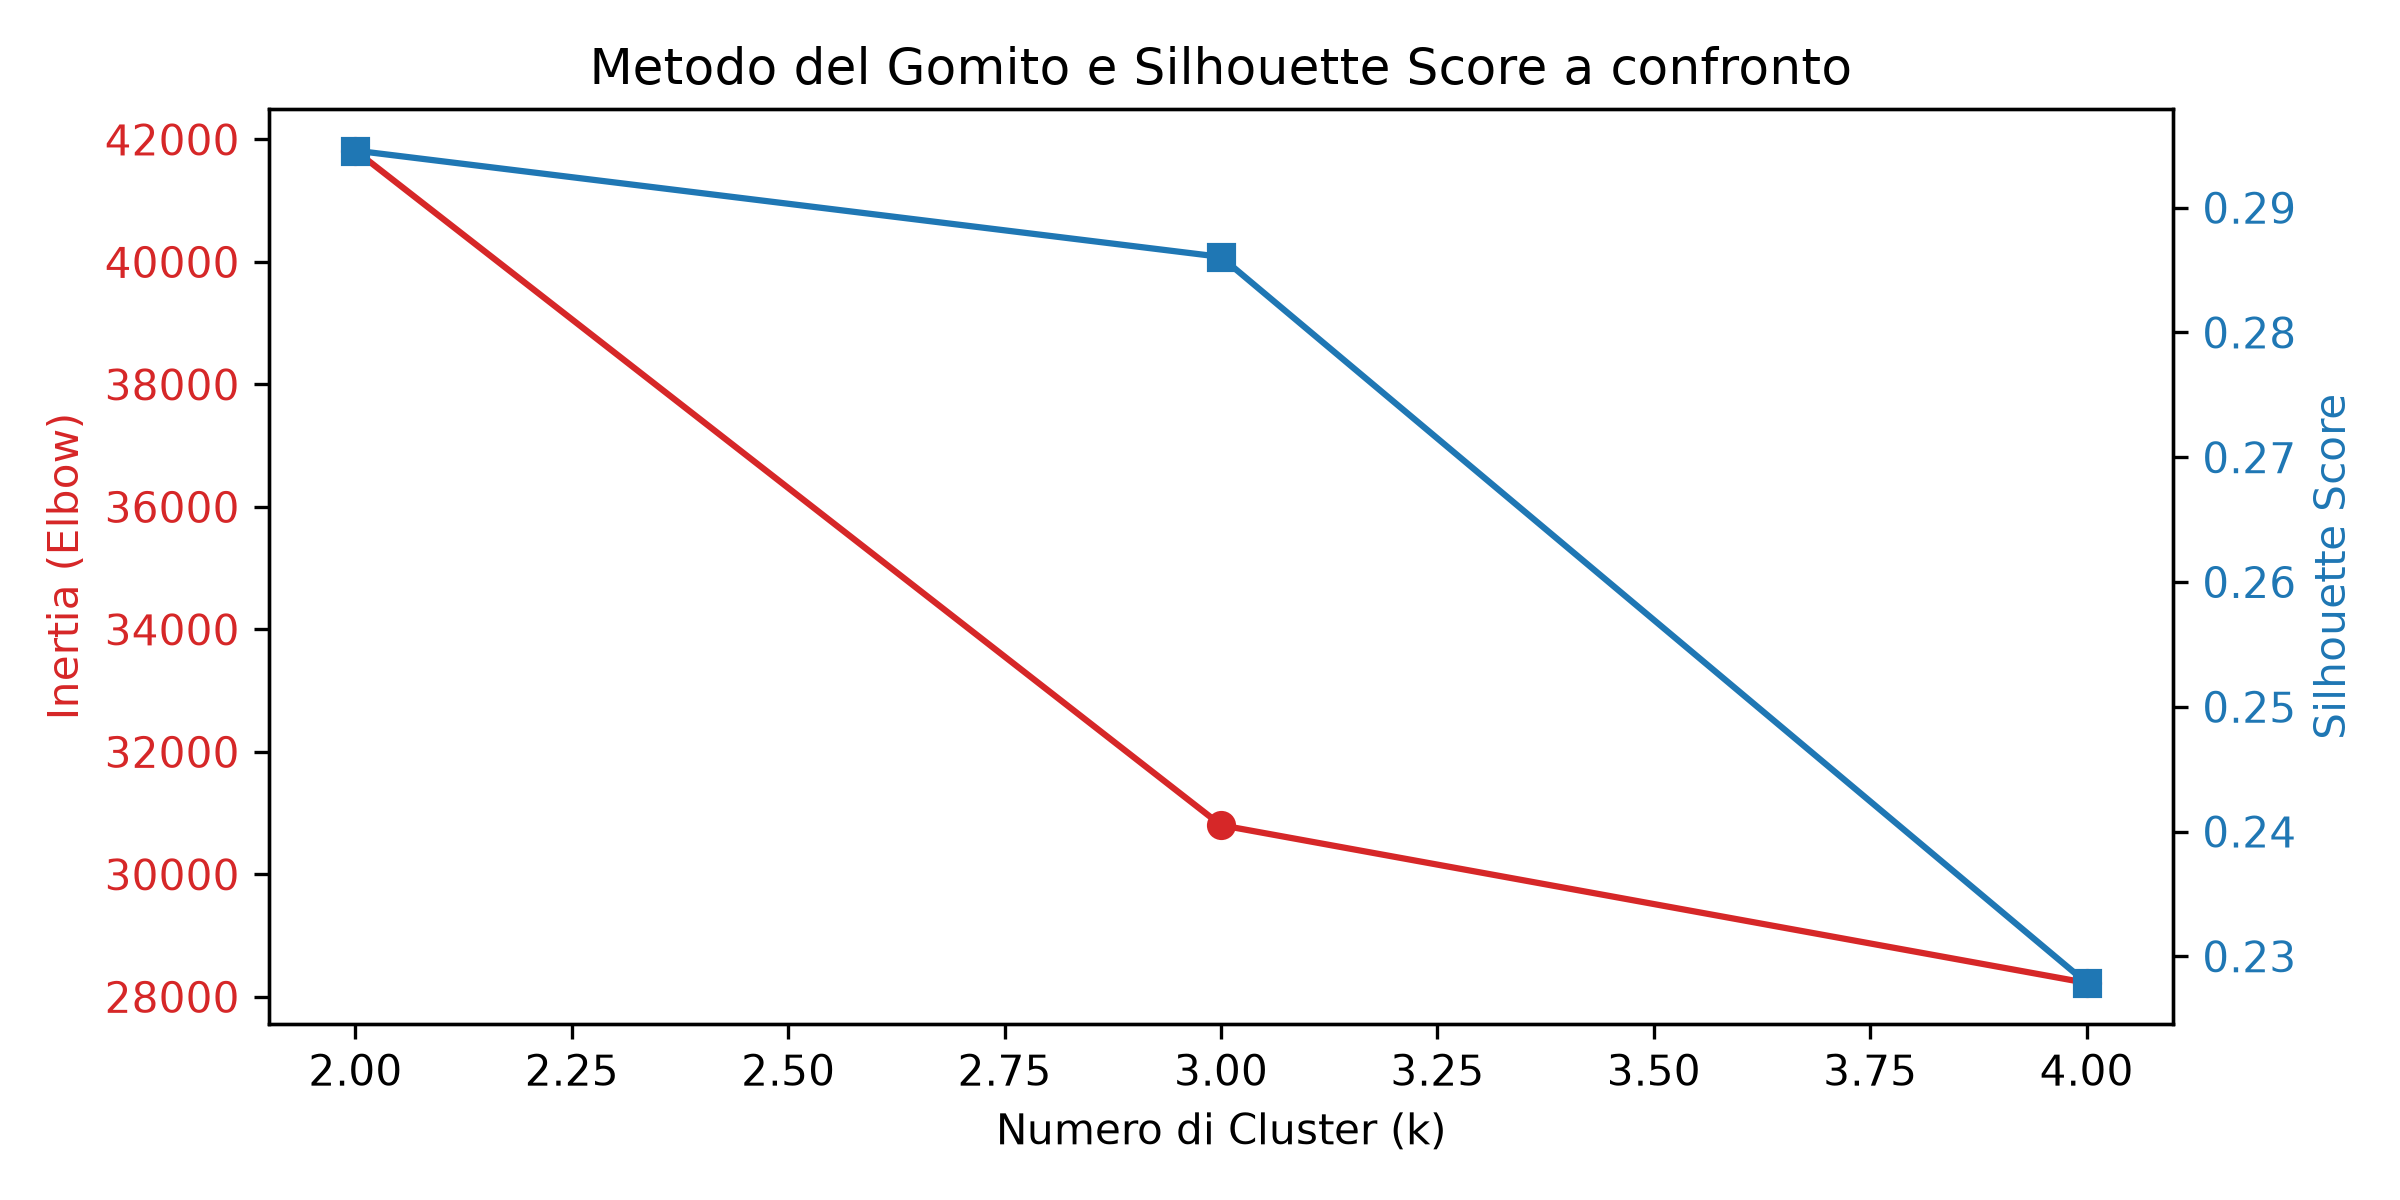
\includegraphics[width=0.7\textwidth]{../grafici/clustering_evaluation.png}
      \begin{center}\scriptsize \textbf{Grafico}: Gomito e Silhouette.\end{center}
    \end{column}
    
    \begin{column}{0.48\textwidth}
      \textbf{I due profili commerciali ($k=2$):}
      \vspace{0.1cm}
      
      \begin{exampleblock}{Cluster 0: Fedeli a basso consumo}
        \scriptsize
        \begin{itemize}
          \item \textbf{Spesa / Mesi}: 21.08 \$ / 30.5 mesi (medie).
          \item \textbf{Contratto}: Pluriennali (stabili).
          \item \textbf{Tasso di Churn}: \textbf{7.40\%} (estremamente sicuro).
        \end{itemize}
      \end{exampleblock}
      
      \begin{alertblock}{Cluster 1: Ad alta spesa e volatili}
        \scriptsize
        \begin{itemize}
          \item \textbf{Spesa / Mesi}: 76.84 \$ / 32.9 mesi (medie).
          \item \textbf{Contratto}: Mensile flessibile.
          \item \textbf{Tasso di Churn}: \textbf{31.83\%} (rischio 4 volte superiore).
        \end{itemize}
      \end{alertblock}
    \end{column}
  \end{columns}
\end{frame}
\begin{frame}{4. I Modelli di Predizione e gli Scenari}
  \textbf{Abbiamo addestrato 3 classificatori con filosofie differenti:}
  \vspace{0.1cm}
  
  \begin{columns}[t]
    \begin{column}{0.31\textwidth}
      \begin{block}{1. Regressione Logistica}
        \scriptsize
        \textbf{Baseline lineare.}\\
        Calcola l'impatto delle caratteristiche del cliente e le mappa in una probabilità tramite la curva \textbf{Sigmoide}.
      \end{block}
    \end{column}
    \begin{column}{0.31\textwidth}
      \begin{block}{2. Albero di Decisione}
        \scriptsize
        \textbf{Modello White-Box.}\\
        Crea regole logiche gerarchiche (IF-THEN). Trova gli split migliori per massimizzare l'omogeneità dei gruppi (Gini).
      \end{block}
    \end{column}
    \begin{column}{0.31\textwidth}
      \begin{block}{3. MLP (Rete Neurale)}
        \scriptsize
        \textbf{Modello Black-Box.}\\
        Rete a strati densi per catturare relazioni complesse ed effetti combinati delle caratteristiche.
      \end{block}
    \end{column}
  \end{columns}
  
  \vspace{0.3cm}
  \textbf{I due scenari di addestramento messi a confronto:}
  \vspace{0.1cm}
  
  \begin{columns}
    \begin{column}{0.48\textwidth}
      \begin{block}{Scenario A: Senza Cluster}
        \scriptsize
        I modelli usano solo le feature originali del dataset (dati commerciali e anagrafici preelaborati).
      \end{block}
    \end{column}
    \begin{column}{0.48\textwidth}
      \begin{block}{Scenario B: Con Cluster (Modello Ibrido)}
        \scriptsize
        Aggiungiamo all'input il \textbf{cluster di appartenenza (0 o 1)} di $k$-Means, per valutarne il valore informativo.
      \end{block}
    \end{column}
  \end{columns}
\end{frame}

% Slide 5b: Funzionamento Concettuale dei Modelli
\begin{frame}{4.1 Come Funzionano i Modelli? (Concetti Chiave)}
  \textbf{Ogni classificatore elabora i dati con una logica differente:}
  \vspace{0.2cm}
  
  \begin{columns}[t]
    \begin{column}{0.32\textwidth}
      \begin{block}{Regressione Logistica}
        \scriptsize
        \textbf{Logica Probabilistica:}\\
        \begin{itemize}
          \item Pesa l'influenza di ciascuna variabile sul rischio di abbandono.
          \item Calcola una probabilità complessiva che il cliente se ne vada.
          \item Classifica come "a rischio" se supera la soglia del 50\%.
        \end{itemize}
      \end{block}
    \end{column}
    
    \begin{column}{0.32\textwidth}
      \begin{block}{Albero di Decisione}
        \scriptsize
        \textbf{Logica a Regole (IF-THEN):}\\
        \begin{itemize}
          \item Divide ricorsivamente i dati ponendo domande basate su soglie (es. \textit{tenure} $\le 10$ mesi).
          \item Cerca lo split che crea i gruppi più omogenei e separati.
          \item Struttura visiva trasparente e intuitiva per le scelte aziendali.
        \end{itemize}
      \end{block}
    \end{column}
    
    \begin{column}{0.32\textwidth}
      \begin{block}{Rete Neurale (MLP)}
        \scriptsize
        \textbf{Logica Multi-Strato:}\\
        \begin{itemize}
          \item Simula una rete di neuroni organizzata in vari livelli.
          \item Combina le variabili per apprendere relazioni non lineari complesse.
          \item Regola continuamente le connessioni per correggere gli errori di stima.
        \end{itemize}
      \end{block}
    \end{column}
  \end{columns}
\end{frame}

% Slide 6: Risultati Sperimentali
\begin{frame}{5. Tabella dei Risultati}
  Confronto tra lo Scenario \textbf{Senza Cluster} e lo Scenario \textbf{Con Cluster} (aggiunto come feature).
  \vspace{0.2cm}
  \begin{table}
    \centering
    \caption{Accuratezza, Recall (Richiamo dei clienti a rischio) e AUC su Train e Test.}
    \resizebox{0.9\textwidth}{!}{
      \begin{tabular}{llcccccc}
        \toprule
         & & \multicolumn{2}{c}{\textbf{Accuracy}} & \multicolumn{2}{c}{\textbf{Recall}} & \multicolumn{2}{c}{\textbf{AUC}} \\
        \cmidrule(lr){3-4} \cmidrule(lr){5-6} \cmidrule(lr){7-8}
        \textbf{Modello} & \textbf{Feature Scenario} & \textbf{Train} & \textbf{Test} & \textbf{Train} & \textbf{Test} & \textbf{Train} & \textbf{Test} \\
        \midrule
        Logistic Regression & Senza Cluster & 0.8053 & 0.8062 & 0.5485 & 0.5588 & 0.8492 & 0.8422 \\
        Logistic Regression & Con Cluster & 0.8051 & 0.8055 & 0.5485 & 0.5588 & 0.8492 & 0.8423 \\
        \midrule
        Decision Tree & Senza Cluster & 0.8023 & 0.7942 & 0.5612 & 0.5401 & 0.8476 & 0.8267 \\
        Decision Tree & Con Cluster & 0.8023 & 0.7942 & 0.5612 & 0.5401 & 0.8476 & 0.8267 \\
        \midrule
        Multi-Layer Perceptron (MLP) & Senza Cluster & 0.9143 & 0.7495 & 0.7813 & 0.4278 & 0.9656 & 0.7844 \\
        \rowcolor{unimeblue!10}
        Multi-Layer Perceptron (MLP) & Con Cluster & 0.9104 & 0.7360 & 0.9097 & \textbf{0.5829} & 0.9722 & 0.7846 \\
        \bottomrule
      \end{tabular}
    }
  \end{table}
  \vspace{0.1cm}
  \begin{itemize}
    \item \textbf{Cosa notare:} L'MLP con l'aggiunta del cluster fa salire la Recall di Test del \textbf{+15.5\%} (da 0.4278 a 0.5829).
  \end{itemize}
\end{frame}

% Slide 7: Albero di Decisione (Visualizzazione)
\begin{frame}{6. Interpretazione dell'Albero di Decisione}
  \footnotesize
  \begin{columns}
    \begin{column}{0.52\textwidth}
      \textbf{Significato dei Colori:}
      \begin{itemize}
        \item \textbf{Nodi Blu}: Clienti fedeli (No Churn).
        \item \textbf{Nodi Arancioni}: Clienti a rischio (Yes Churn).
        \item \textbf{Intensità}: Colori più scuri indicano decisioni più nette e omogenee.
      \end{itemize}
      \vspace{0.15cm}
      
      \textbf{Le 3 Regole Chiave individuate:}
      \begin{itemize}
        \item \textbf{1. Tipo di Contratto}: È lo split iniziale più importante. I contratti mensili sono molto più instabili.
        \item \textbf{2. Mesi di permanenza (Tenure)}: Chi ha un contratto mensile ed è iscritto da poco è nella fascia a rischio massimo.
        \item \textbf{3. Servizi \& Spesa}: Fibra ottica e costi mensili alti aumentano la volatilità dei clienti.
      \end{itemize}
    \end{column}
    \begin{column}{0.45\textwidth}
      \centering
      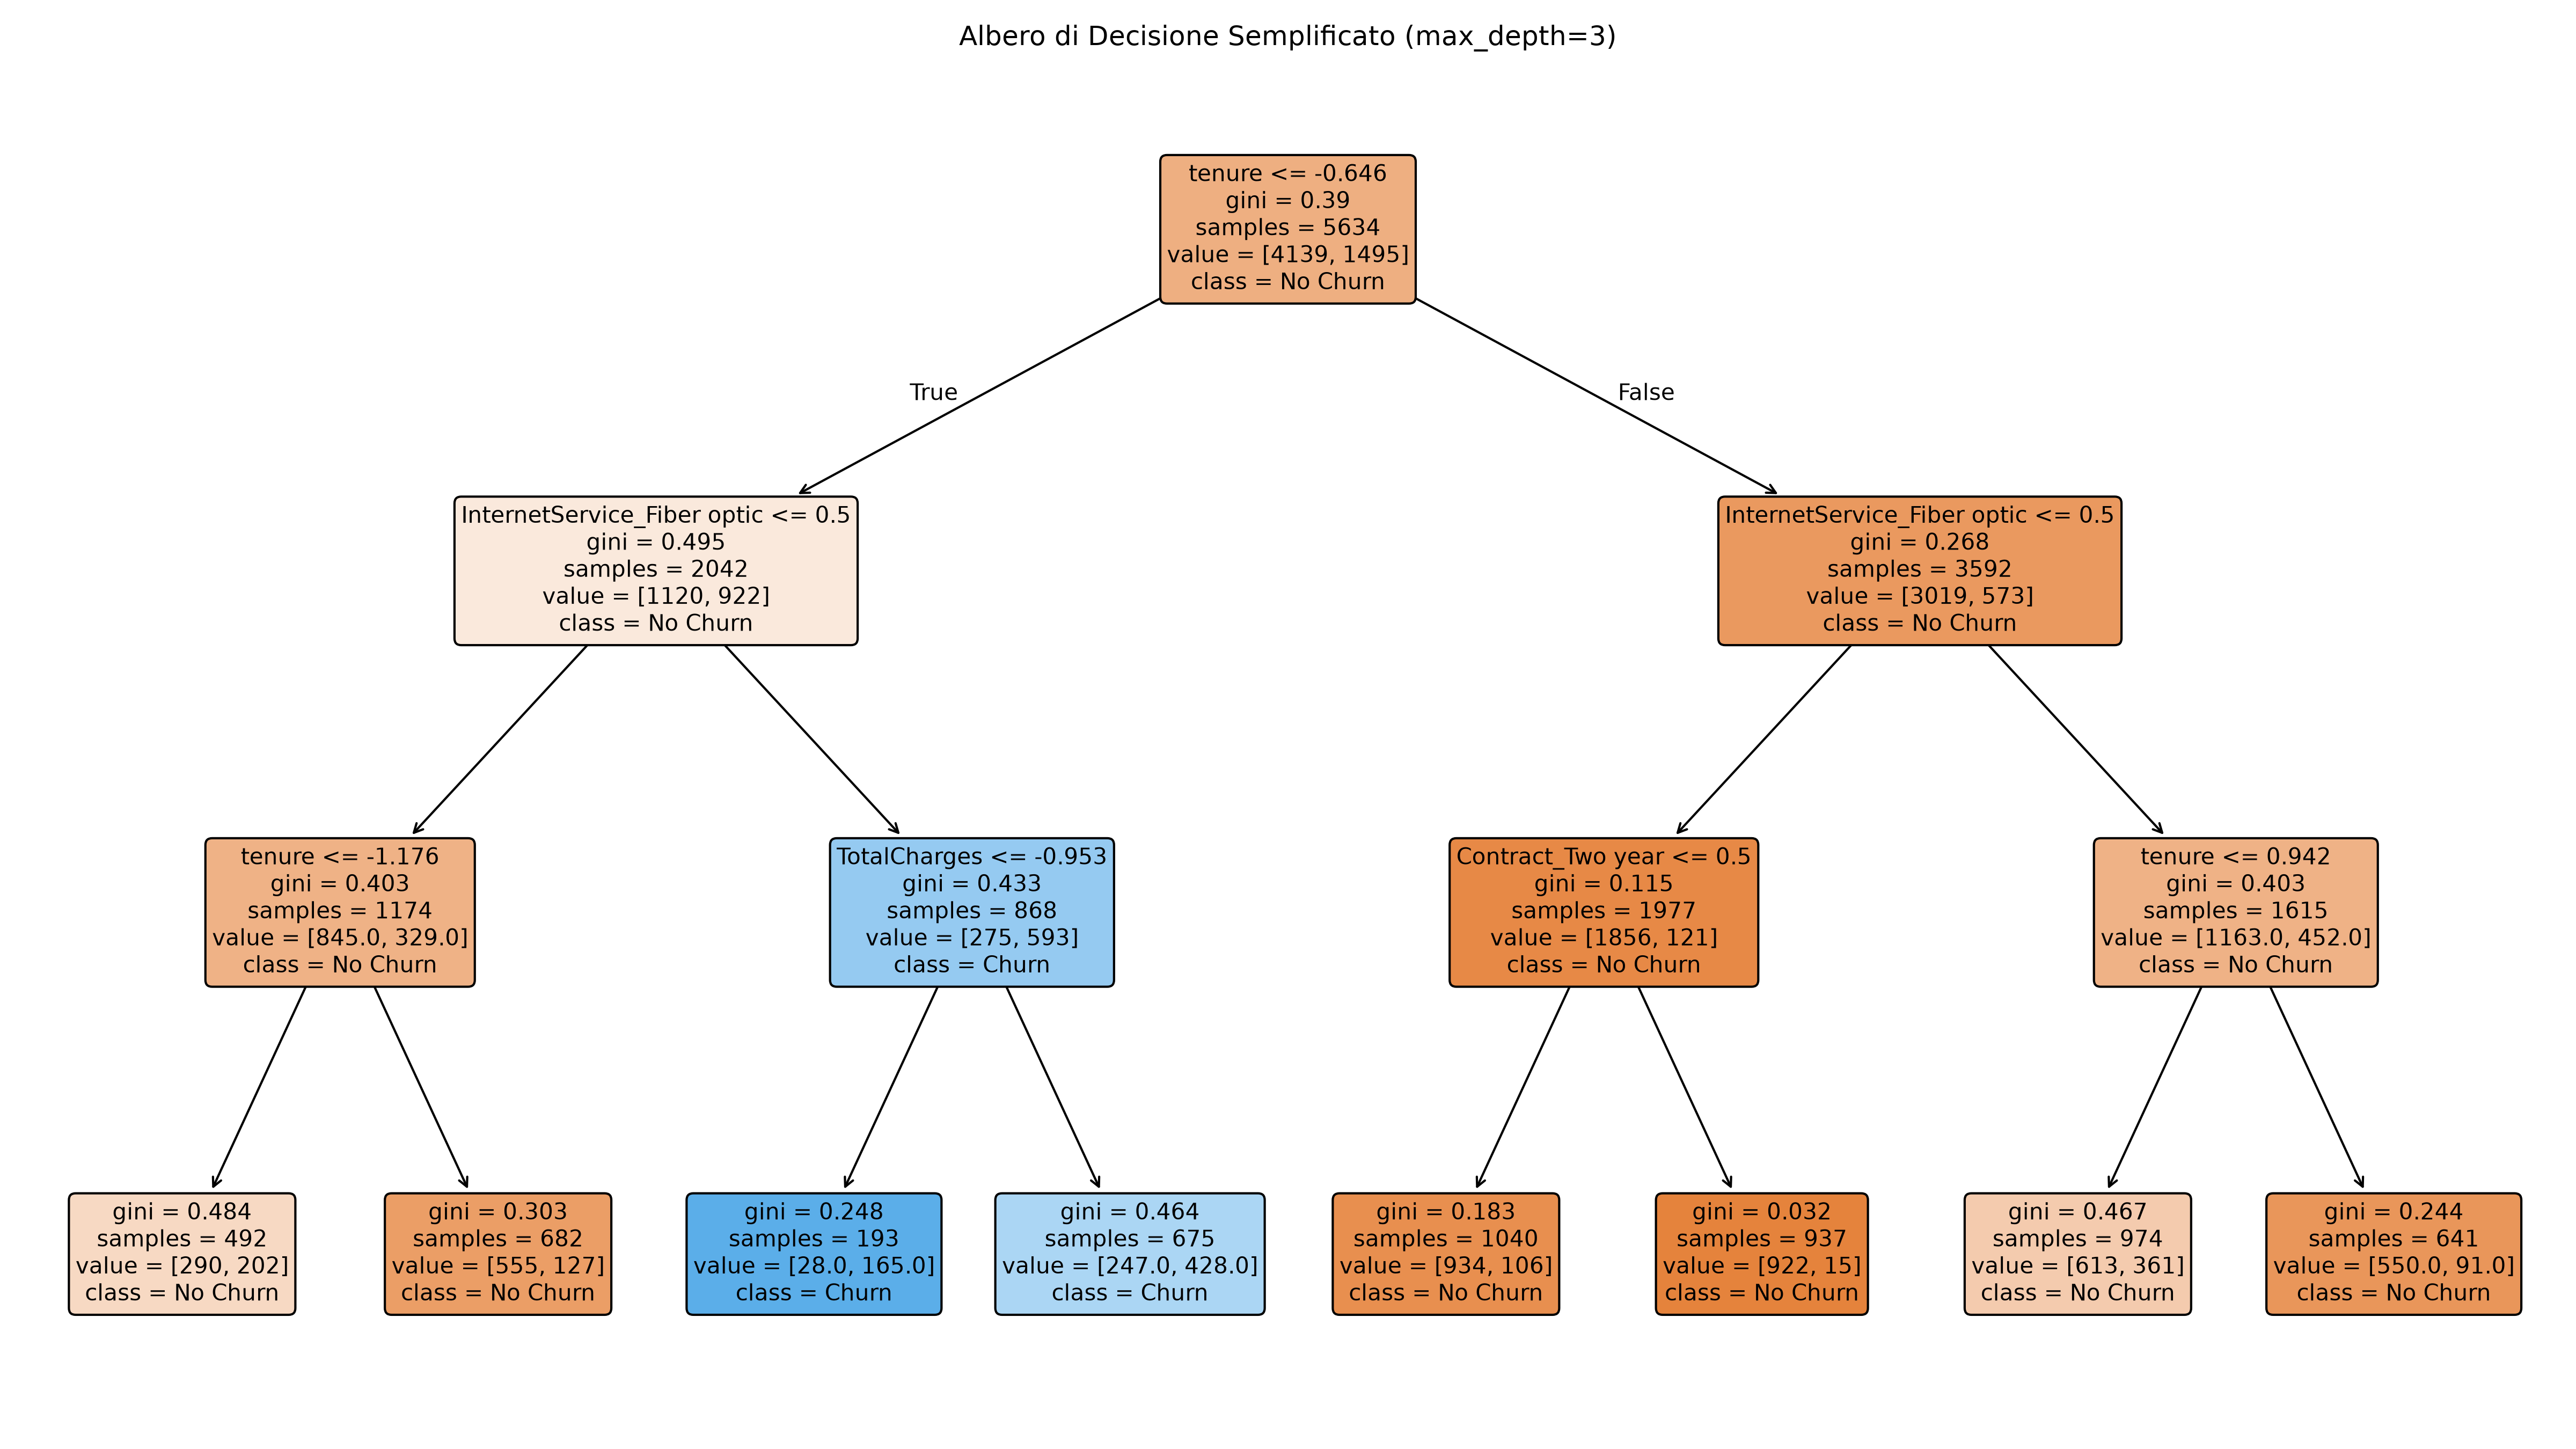
\includegraphics[width=\textwidth]{../grafici/decision_tree_vis.png}
      \begin{center}\scriptsize \textbf{Grafico}: Regole dell'albero.\end{center}
    \end{column}
  \end{columns}
\end{frame}

% Slide 8: Overfitting dell'MLP e Importanza Feature
\begin{frame}{7. Diagnostica dei Modelli e Indizi Chiave}
  \footnotesize
  \begin{columns}
    \begin{column}{0.52\textwidth}
      \textbf{Capire gli Errori dei Modelli:}
      \begin{itemize}
        \item \textbf{Underfitting (Studiare troppo poco)}: Non è il nostro caso. I modelli sono in grado di catturare le regole di base dei dati ($\approx 80\%$ di accuratezza).
        \item \textbf{Overfitting (Studiare a memoria)}: Colpisce la Rete Neurale (MLP). Ottiene il 91\% di risposte corrette in addestramento, ma cala al 73.6\% su dati nuovi perché "impara a memoria" i dettagli.
      \end{itemize}
      \vspace{0.15cm}
      
      \textbf{L'utilità reale del Cluster:}
      \begin{itemize}
        \item Anche se la Rete Neurale soffre di overfitting, l'uso del \textbf{Cluster} come indizio extra la guida nel focalizzarsi sui clienti giusti: la sua capacità di trovarli (Recall) sale del \textbf{+15.5\%} (da 42.8\% a 58.3\%).
      \end{itemize}
    \end{column}
    \begin{column}{0.45\textwidth}
      \centering
      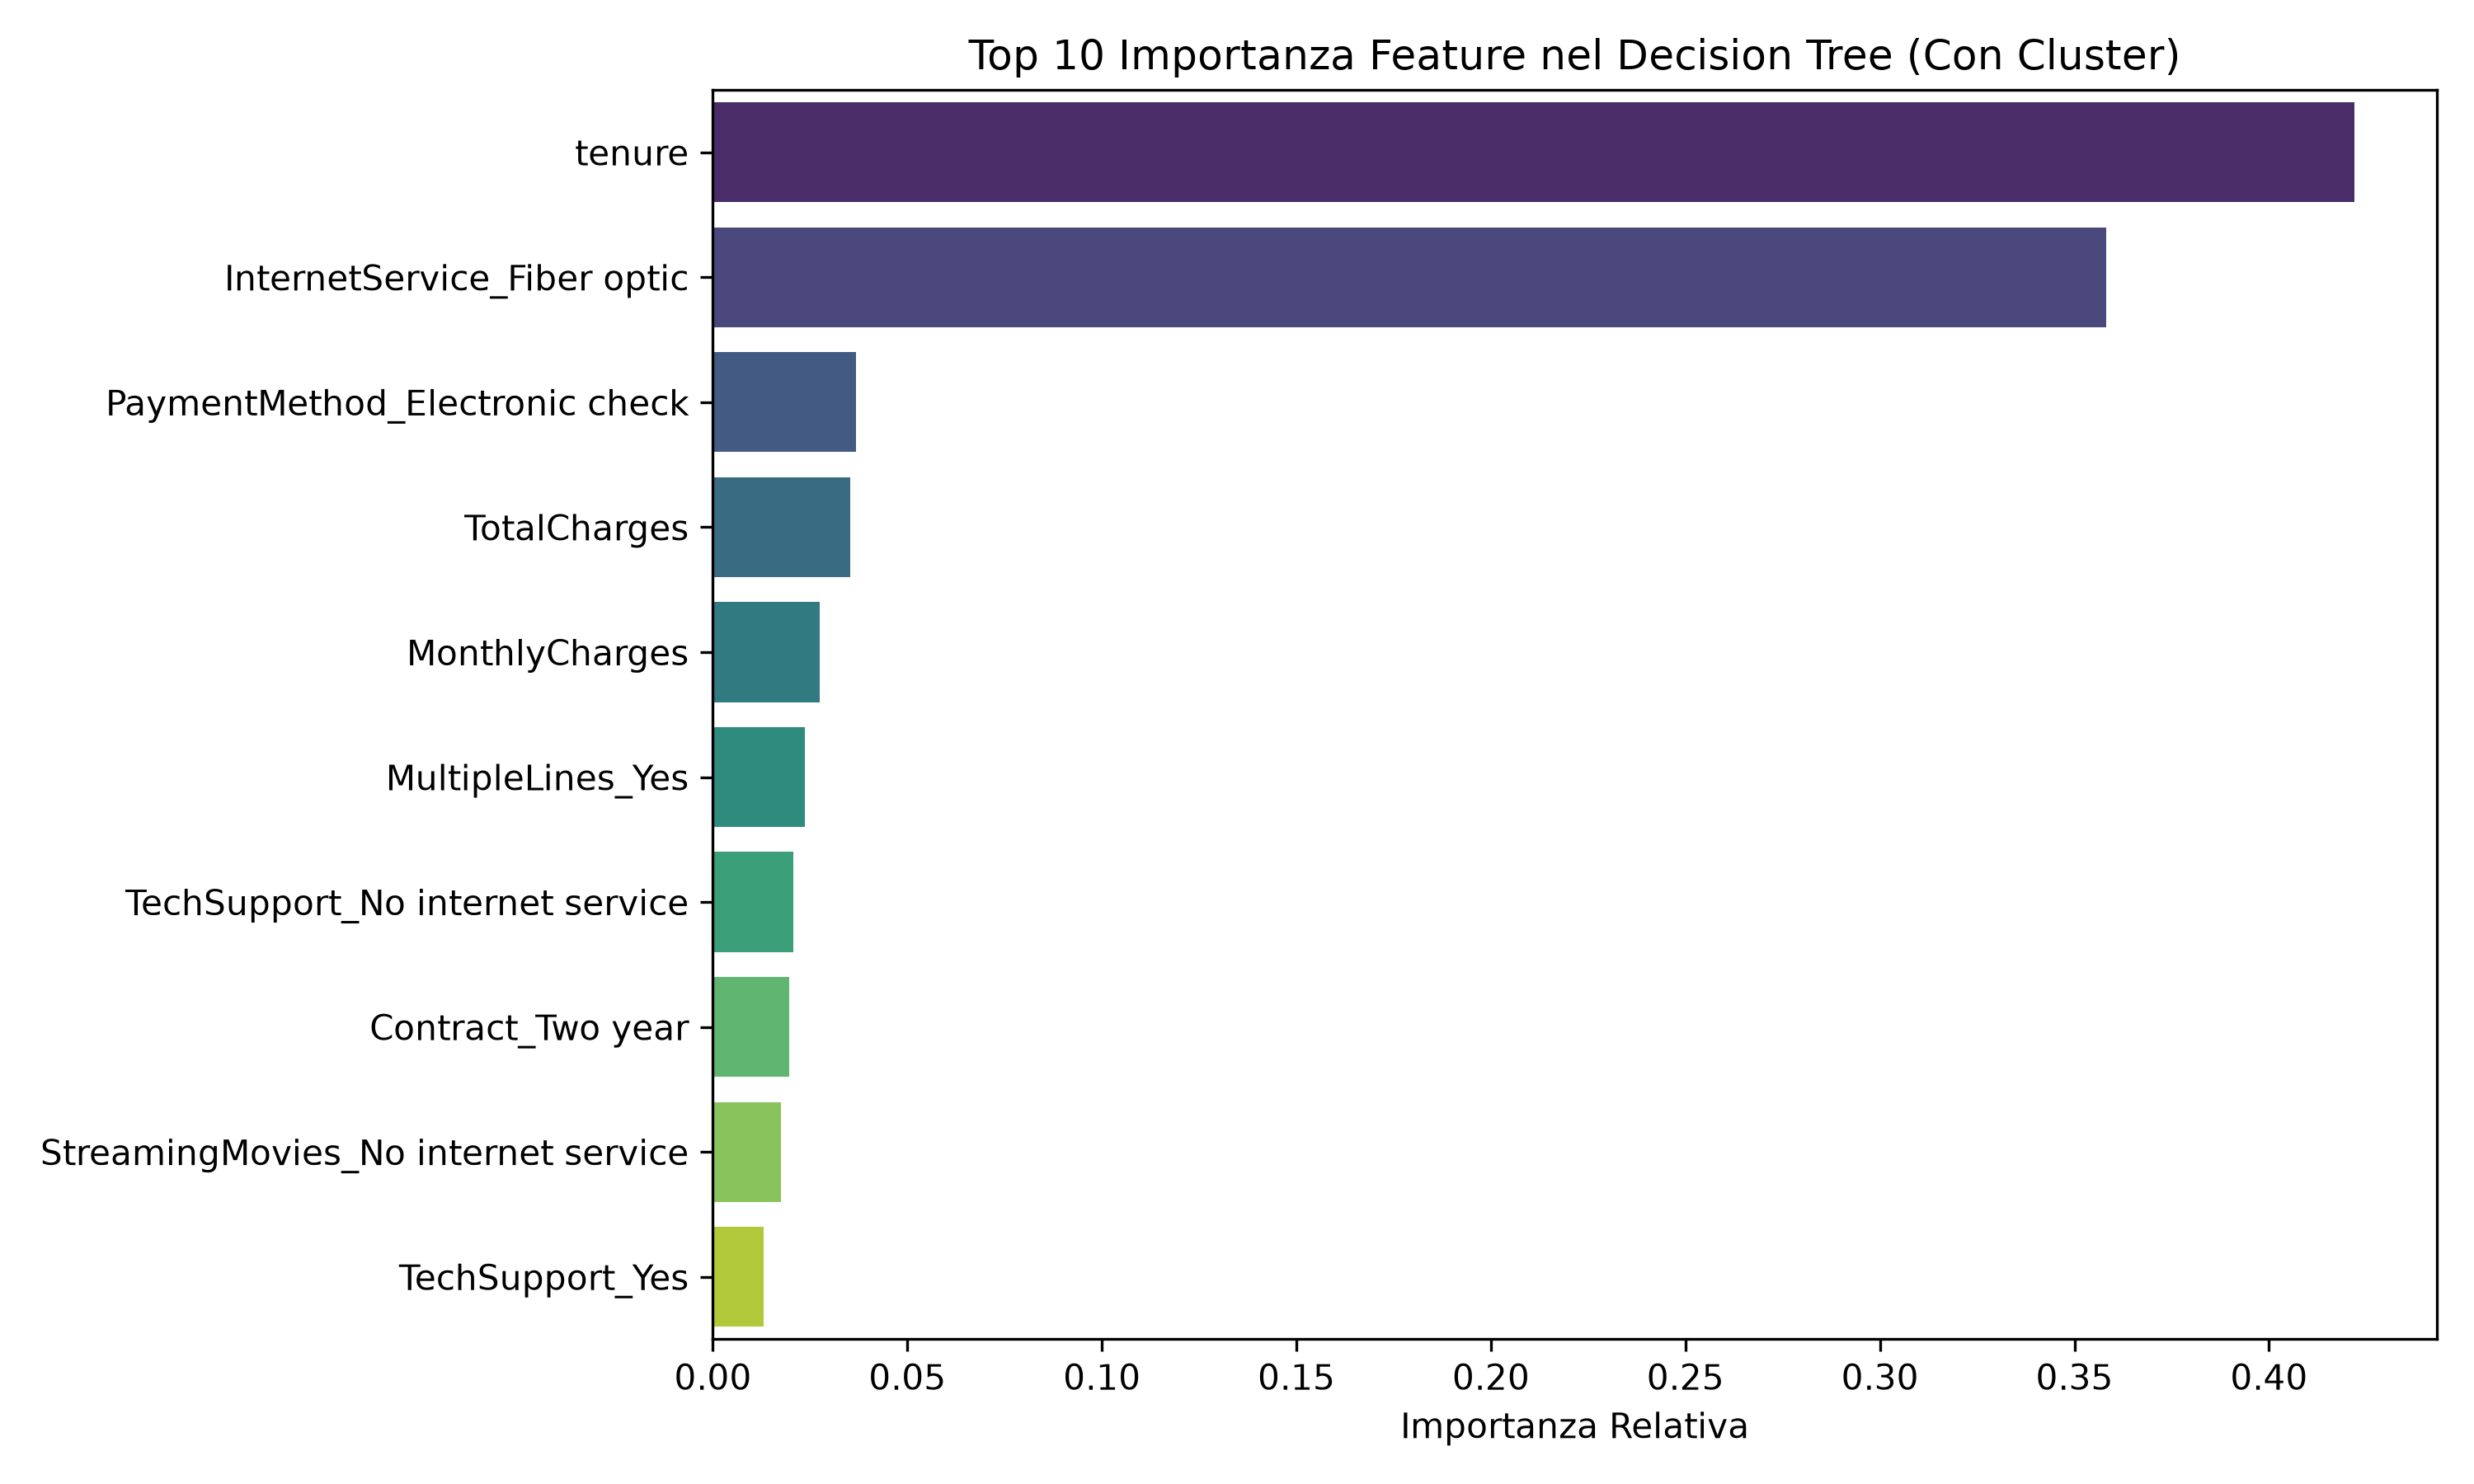
\includegraphics[width=\textwidth]{../grafici/feature_importances.png}
      \begin{center}\scriptsize \textbf{Grafico}: I 10 indizi più importanti. I mesi di permanenza (\textit{tenure}) e la fibra ottica guidano la decisione.\end{center}
    \end{column}
  \end{columns}
\end{frame}

% Slide 9: Conclusioni
\begin{frame}{8. Cosa impariamo da questo Progetto?}
  \footnotesize
  \textbf{Le Lezioni del Progetto:}
  \begin{itemize}
    \item \textbf{Utilità del Clustering}: Il $k$-Means ha estratto profili commerciali chiari (fedeli a bassa spesa vs. volatili ad alta spesa) utili per definire strategie aziendali mirate.
    \item \textbf{Valore del Modello Ibrido}: Inserire il Cluster come feature ha potenziato la Rete Neurale (MLP), aumentandone la Recall sul test del \textbf{+15.5\%} (scovando molti più clienti in partenza).
    \item \textbf{Scelta del Modello}: L'Albero di Decisione è preferibile per la trasparenza aziendale delle sue regole di split, mentre l'MLP ha potenzialità maggiori ma richiede controllo sull'overfitting.
  \end{itemize}
  \vspace{0.15cm}
  
  \textbf{Sviluppi Futuri (Miglioramento dei Modelli Esistenti):}
  \begin{itemize}
    \item \textbf{Regolarizzazione dell'MLP}: Introdurre penalizzazioni (L2) o arresto anticipato per ridurre l'overfitting e stabilizzare l'accuratezza di test.
    \item \textbf{Bilanciamento dei Dati}: Gestire lo sbilanciamento delle classi (es. tramite tecniche come SMOTE) per addestrare i modelli su campioni di churn più equilibrati.
  \end{itemize}
  \vspace{0.25cm}
  \centering
  \textbf{\large Grazie per l'attenzione!}
\end{frame}

\end{document}
